\chapter{Implementação do Cliente}
\label{chap:impl}
Para que fosse possível que implementássemos um agente de inteligência artificial que
jogasse uma versão simplificada de Magic, era essencial que conhecêssemos em detalhe a
plataforma onde o jogo estaria rodando, e para isso implementamos do zero uma versão do
jogo com as especifidades desejadas usando a linguagem Python.

O programa é composto de quatro classes principais: \texttt{Game}, \texttt{Player}, \texttt{Card}
e \texttt{Permanent}, representando o Jogo, Jogadores, Cartas e Permanentes (como são tratadas as
cartas de Terreno e Criatura uma vez que estão em jogo) respectivamente. A seguir vamos falar de
cada uma destas classes entrando em detalhes nas principais características.

\section{\texttt{class Card:}}
A classe \texttt{Card} representa as cartas do jogo. Os objetos que estarão presentes nas mãos,
decks e cemitérios dos jogadores serão classes que herdam desta classe. Seus atributos representam
características presentes em todas as cartas. Para exemplificar os atributos, usaremos as cartas mostradas no capítulo anterior: Volcanic Hammer e Angel of Mercy. Os atributos a seguir são comuns a todos os tipos de carta, e por isso estão presentes na
classe Card:

\begin{itemize}
  \item\texttt{name}: Uma string representando o nome da carta, por exemplo ``Volcanic Hammer''
  ou ``Angel of Mercy''.
  \item\texttt{cost}: Uma string representando o custo de mana da carta, usando a mesma notação
  presente nas cartas, com W, U, B, R e G representando os símbolos de mana $\vcenter{\hbox{
\includegraphics[scale=0.015]{picstcc/W.png}}}$ (Branco), $\vcenter{\hbox{
\includegraphics[scale=0.015]{picstcc/U.png}}}$ (Azul),
  $\vcenter{\hbox{
\includegraphics[scale=0.015]{picstcc/B.png}}}$ (Preto),
  $\vcenter{\hbox{
\includegraphics[scale=0.015]{picstcc/R.png}}}$ (Vermelho) e $\vcenter{\hbox{
\includegraphics[scale=0.015]{picstcc/G.png}}}$ (Verde) respectivamente. No caso de Volcanic Hammer, o custo é ``1R'' e no de Angel of Mercy, ``4W''.
  \item\texttt{supertype}: Uma string representando o supertipo da carta. No nosso programa,
  o único supertipo que irá aparecer é \texttt{'Basic'}``Basic'', que identifica os terrenos básicos, mas essa
  informação não é relevante para o programa. Estamos representando essa informação principalmente por formalidade para que o programa siga a mesma estrutura de tipos descrita nas regras do jogo. Nem Volcanic Hammer nem Angel of Mercy
  possuem supertipos, portanto este atributo é representado pela string vazia.
  \item\texttt{ctype}: Uma string que representa o tipo da carta. Angel of Mercy recebe o tipo
  \texttt{'Creature'} e Volcanic Hammer,\texttt{'Sorcery'}. Diferentemente de supertipo ou subtipo,
  este é um atributo que nunca estará vazio em uma carta.
  \item\texttt{subtype}: Uma string que representa o subtipo da carta. O subtipo serve para que
  algumas cartas tenham uma informação adicional que possa ser usada para ações dentro do jogo.
  Volcanic Hammer não tem subtipo, enquanto o subtipo de Angel of Mercy recebe \texttt{'Angel'}.
  \item\texttt{text}: Uma string representando o texto da carta. Essa string serve somente para
  interface com o jogador. O texto de Volcanic Hammer é ``Volcanic Hammer deals 3 damage to target
  creature or player.'' enquanto o de Angel of Mercy é ``Flying. When Angel of Mercy enters the
  battlefield, you gain 3 life. 3/3''.
  \item\texttt{targets}: Uma lista contendo tuplas com as possibilidades de alvo que a carta
  pode ter. Angel of Mercy não tem alvos, e portanto sua lista de alvos é vazia. Volcanic Hammer
  pode dar alvo em criaturas ou jogadores, então sua lista de alvos é
  \texttt{[(``OwnCreature'', ``OpponentCreature'', ``Player'')]}. Separamos criaturas  entre
  criaturas do mesmo dono da carta ou criaturas dos oponentes pois há cartas que só podem ter
  um destes conjuntos como alvo, facilitando a implementação.
  \item\texttt{owner}: O jogador dono da carta. Este atributo é do tipo \texttt{Player}.
\end{itemize}
Para cada carta com nome diferente, há uma classe que herda da classe \texttt{Card} e implementa
as especificidades da carta. Vejamos o código da classe \texttt{VolcanicHammer}, que implementa
a carta Volcanic Hammer:
\begin{figure}
  \begin{Verbatim}[commandchars=\\\{\}]
\PY{k}{class} \PY{n+nc}{VolcanicHammer}\PY{p}{(}\PY{n}{Card}\PY{p}{)}\PY{p}{:}
    \PY{k}{def} \PY{n+nf+fm}{\PYZus{}\PYZus{}init\PYZus{}\PYZus{}}\PY{p}{(}\PY{n+nb+bp}{self}\PY{p}{,} \PY{n}{owner}\PY{p}{)}\PY{p}{:}
        \PY{n+nb+bp}{self}\PY{o}{.}\PY{n}{name} \PY{o}{=} \PY{l+s+s2}{\PYZdq{}}\PY{l+s+s2}{Volcanic Hammer}\PY{l+s+s2}{\PYZdq{}}
        \PY{n+nb+bp}{self}\PY{o}{.}\PY{n}{cost} \PY{o}{=} \PY{l+s+s2}{\PYZdq{}}\PY{l+s+s2}{1R}\PY{l+s+s2}{\PYZdq{}}
        \PY{n+nb+bp}{self}\PY{o}{.}\PY{n}{supertype} \PY{o}{=} \PY{l+s+s2}{\PYZdq{}}\PY{l+s+s2}{\PYZdq{}}
        \PY{n+nb+bp}{self}\PY{o}{.}\PY{n}{ctype} \PY{o}{=} \PY{l+s+s2}{\PYZdq{}}\PY{l+s+s2}{Sorcery}\PY{l+s+s2}{\PYZdq{}}
        \PY{n+nb+bp}{self}\PY{o}{.}\PY{n}{subtype} \PY{o}{=} \PY{l+s+s2}{\PYZdq{}}\PY{l+s+s2}{\PYZdq{}}
        \PY{n+nb+bp}{self}\PY{o}{.}\PY{n}{text} \PY{o}{=} \PY{l+s+s2}{\PYZdq{}}\PY{l+s+s2}{Volcanic Hammer deals 3 damage to target creature or player.}\PY{l+s+s2}{\PYZdq{}}
        \PY{n+nb+bp}{self}\PY{o}{.}\PY{n}{targets} \PY{o}{=} \PY{p}{[}\PY{p}{[}\PY{l+s+s2}{\PYZdq{}}\PY{l+s+s2}{OwnCreature}\PY{l+s+s2}{\PYZdq{}}\PY{p}{,} \PY{l+s+s2}{\PYZdq{}}\PY{l+s+s2}{OpponentCreature}\PY{l+s+s2}{\PYZdq{}}\PY{p}{,} \PY{l+s+s2}{\PYZdq{}}\PY{l+s+s2}{Player}\PY{l+s+s2}{\PYZdq{}}\PY{p}{]}\PY{p}{]}
        \PY{n+nb+bp}{self}\PY{o}{.}\PY{n}{owner} \PY{o}{=} \PY{n}{owner}

    \PY{k}{def} \PY{n+nf}{effect}\PY{p}{(}\PY{n+nb+bp}{self}\PY{p}{,} \PY{n}{game}\PY{p}{,} \PY{n}{targets}\PY{p}{)}\PY{p}{:}
        \PY{n}{targets}\PY{p}{[}\PY{l+m+mi}{0}\PY{p}{]}\PY{o}{.}\PY{n}{takeDamage}\PY{p}{(}\PY{l+m+mi}{3}\PY{p}{)}
\end{Verbatim}

\end{figure}
Podemos ver que a classe tem o método \texttt{effect()}, que implementa o efeito da carta,
fazendo com que o alvo escolhido sofra três pontos de dano. Vejamos agora a implementação
da carta Angel of Mercy:
\begin{figure}
  
\begin{Verbatim}[commandchars=\\\{\}]
\PY{k}{class} \PY{n+nc}{AngelofMercy}\PY{p}{(}\PY{n}{Card}\PY{p}{)}\PY{p}{:}
    \PY{k}{def} \PY{n+nf+fm}{\PYZus{}\PYZus{}init\PYZus{}\PYZus{}}\PY{p}{(}\PY{n+nb+bp}{self}\PY{p}{,}\PY{n}{owner}\PY{p}{)}\PY{p}{:}
        \PY{n+nb+bp}{self}\PY{o}{.}\PY{n}{name} \PY{o}{=} \PY{l+s+s2}{\PYZdq{}}\PY{l+s+s2}{Angel of Mercy}\PY{l+s+s2}{\PYZdq{}}
        \PY{n+nb+bp}{self}\PY{o}{.}\PY{n}{cost} \PY{o}{=} \PY{l+s+s2}{\PYZdq{}}\PY{l+s+s2}{4W}\PY{l+s+s2}{\PYZdq{}}
        \PY{n+nb+bp}{self}\PY{o}{.}\PY{n}{supertype} \PY{o}{=} \PY{l+s+s2}{\PYZdq{}}\PY{l+s+s2}{\PYZdq{}}
        \PY{n+nb+bp}{self}\PY{o}{.}\PY{n}{ctype} \PY{o}{=} \PY{l+s+s2}{\PYZdq{}}\PY{l+s+s2}{Creature}\PY{l+s+s2}{\PYZdq{}}
        \PY{n+nb+bp}{self}\PY{o}{.}\PY{n}{subtype} \PY{o}{=} \PY{l+s+s2}{\PYZdq{}}\PY{l+s+s2}{Angel}\PY{l+s+s2}{\PYZdq{}}
        \PY{n+nb+bp}{self}\PY{o}{.}\PY{n}{text} \PY{o}{=} \PY{l+s+s2}{\PYZdq{}}\PY{l+s+s2}{Flying. When Angel of Mercy enters the battlefield, you gain 3 life. 3/3}\PY{l+s+s2}{\PYZdq{}}
        \PY{n+nb+bp}{self}\PY{o}{.}\PY{n}{abilities} \PY{o}{=} \PY{p}{[}\PY{l+s+s2}{\PYZdq{}}\PY{l+s+s2}{Flying}\PY{l+s+s2}{\PYZdq{}}\PY{p}{]}
        \PY{n+nb+bp}{self}\PY{o}{.}\PY{n}{targets} \PY{o}{=} \PY{p}{[}\PY{p}{]}
        \PY{n+nb+bp}{self}\PY{o}{.}\PY{n}{owner} \PY{o}{=} \PY{n}{owner}
        \PY{n+nb+bp}{self}\PY{o}{.}\PY{n}{power} \PY{o}{=} \PY{l+m+mi}{3}
        \PY{n+nb+bp}{self}\PY{o}{.}\PY{n}{tou} \PY{o}{=} \PY{l+m+mi}{3}

    \PY{k}{def} \PY{n+nf}{effect}\PY{p}{(}\PY{n+nb+bp}{self}\PY{p}{,} \PY{n}{game}\PY{p}{,} \PY{n}{targets}\PY{p}{)}\PY{p}{:}
        \PY{n+nb+bp}{self}\PY{o}{.}\PY{n}{owner}\PY{o}{.}\PY{n}{gainLife}\PY{p}{(}\PY{l+m+mi}{3}\PY{p}{)}
\end{Verbatim}

\end{figure}
Além dos atributos que citamos anteriormente, Angel of Mercy tem três atributos a mais por
ser do tipo Criatura: \texttt{abilities}, uma lista com as habilidades de combate da criatura;
\texttt{power}, o poder da criatura; e \texttt{tou}, a resistência (toughness) da criatura.
Podemos também ver o efeito da carta, que concede três pontos de vida a seu controlador. O método \texttt{effect} de cada carta é chamado quando esta é jogada, tendo consequências distintas para cada caso.

\section{\texttt{class Permanent:}}
A classe \texttt{Permanent} serve para representar as cartas uma vez que foram jogadas
e estão no campo de batalha. Seus atributos são os seguintes:
\begin{itemize}
  \item\texttt{card}: A carta que criou a permanente. Ela contém informações relevantes
  para a construção do objeto e é ela, e não a permanente, que será colocada no cemitério
  caso deixe o campo de batalha.
  \item\texttt{abilities}: Uma cópia do atributo \texttt{abilities} da carta. É necessário
  que esse atributo seja armazenado separadamente ao da carta, pois uma vez em jogo, a
  permanente pode ganhar ou perder habilidades.
  \item\texttt{ctype}: O tipo da permanente, conforme descrito na carta que a criou.
  \item\texttt{owner}: O jogador dono da permanente, que será o mesmo que possúi a carta.
  \item\texttt{controller}: O jogador controlador da permanente. Normalmente ele será o dono,
  mas há efeitos que mudam o jogador que controla uma permanente.
  \item\texttt{tapped}: Um atributo booleano que indica se a permanente está virada ou
  desvirada.
  \item\texttt{sick}: Um atributo booleano que indica se a permanente está
  \textit{enjoada}\footnote{Permanentes entram em jogo com \textit{enjoo de invocação}, o que
  indica que caso ela seja uma criatura, não poderá atacar. O enjoo de uma permanente acaba no
  começo do turno de seu controlador.} ou não.
  \item\texttt{destroyed}: Um atributo booleano que indica se a permanente foi destruída ou não.
  Permanentes destruídas são colocadas no cemitério de seu controlador durante as checagens do jogo.
  \item\texttt{ID}: Um inteiro que serve como identificador único entre permanentes. Ele serve,
  por exemplo, para diferenciar permanentes que tenham sido criadas a partir de cartas iguais.
\end{itemize}
Estes atributos são alterados a partir dos métodos da classe, que não entraremos em detalhes.

Há duas classes que herdam da classe \texttt{Permanent}: \texttt{Land} e \texttt{Creature}.
\texttt{Land} é a classe que representa terrenos. A única diferença desta classe para a classe
mãe é que os métodos de virar e desvirar manipulam um atributo do jogador controlador: a quantidade
de terrenos desvirados controlados por aquele jogador. A classe \texttt{Creature} tem alguns
atributos a mais:
\begin{itemize}
  \item\texttt{power}: Um inteiro que representa o poder da criatura.
  \item\texttt{tou}: Um inteiro que representa a resistência da criatura.
  \item\texttt{curPower}: Um inteiro que representa o poder atual da criatura. Existem efeitos
  que modificam o poder com duração limitada a um turno. Nestes casos, o poder volta a ser o
  poder armazenado no atributo \texttt{power} quando o próximo turno começar.
  \item\texttt{curTou}: Um inteiro que representa a resistência atual da criatura. Análogo ao
  atributo \texttt{curPower} relativo à resistência da criatura.
  \item\texttt{attacking}: Um atributo booleano que representa se a criatura está atacando
  ou não.
  \item\texttt{blocking}: Um atributo booleano que representa se a criatura está bloqueando
  ou não.
  \item\texttt{damage}: Um inteiro que armazena a quantidade de dano sofrida pela criatura até
  o presente momento. No início de cada turno, este atributo volta a ter o valor $0$.
  \item\texttt{currentAbilities}: Análogo ao atributo \texttt{curPower} para as habilidades.
\end{itemize}
Criaturas têm alguns métodos especiais que possibilitam com que elas realizem ações dentro
do jogo, como atacar ou causar dano, mas não entraremos em detalhes.

\section{\texttt{class Game:}}
A classe \texttt{Game} representa um jogo em andamento. Devido à complexidade da classe, entrar
em detalhes iria mudar o foco do trabalho, então não iremos descrever todos os métodos e atributos
da classe. Há um método chamado \texttt{turnRoutine()} que é chamado repetidamente até que o jogo
termine. Ele executa as ações iniciais e finais do turno (como fazer com que o jogador ativo compre
uma carta no começo do turno e limpar o dano das criaturas no final do turno) e chama os métodos de
fase principal e de combate, que permitem que os jogadores joguem as cartas da mão, ataquem e
bloqueiem.
\vskip1ex
Além disso, há alguns métodos para definir quais são as ações legais para um jogador e para realizar
as chamades \textit{ações baseadas no estado}, que são ações performadas pelo jogo sempre que uma
certa condição baseada no estado do jogo se torna verdade (por exemplo, destruir criaturas com dano
igual ou superior à resistência, fazer com que jogadores com $0$ ou menos pontos de vida percam o
o jogo, e assim por diante). O método que cuida disso é \texttt{checkSBA()} (de ``state based actions''),
chamado pela classe \texttt{Game} nos seguintes momentos:
\begin{itemize}
  \item No início e fim de cada fase.
  \item Após toda ação de Fase Principal.
  \item Durante etapas de atribuição de dano no Combate.
\end{itemize}
\texttt{Game} é responsável por chamar métodos que requerem a decisão do jogador.
\section{\texttt{class Player:}}
A classe \texttt{Player} representa um jogador na partida. Seus atributos são:
\begin{itemize}
  \item\texttt{name}: Uma string representando o nome do jogador. Não tem nenhuma função
  dentro do jogo. Serve para identificar os jogadores na saída.
  \item\texttt{life}: Um inteiro representando o valor atual do total de pontos de vida
  do jogador.
  \item\texttt{hand}: Uma lista de objetos do tipo \texttt{Card}, representando as cartas
  na mão do jogador.
  \item\texttt{library}: Uma lista de objetos do tipo \texttt{Card}, representando as cartas
  no deck\footnote{Dentro do jogo, o deck recebe o nome de \textit{Grimório}, ou \textit{Library},
  em inglês.} do jogador.
  \item\texttt{lose}: Um atributo booleano para identificar se o jogador perdeu o jogo. Este
  atributo é utilizado pela classe \texttt{Game} para decidir se o jogo acabou ou não.
  \item\texttt{ID}: Um inteiro representando um identificador único para o jogador, de maneira
  similar à que acontece com as permanentes.
  \item\texttt{creatures}: Uma lista de objetos da classe \texttt{Creature} com todas as
  criaturas controladas pelo jogador.
  \item\texttt{lands}: Uma lista de objetos da classe \texttt{Land} com todos os terrenos
  controlados pelo jogador.
  \item\texttt{active}: Um atributo booleano que indica se o jogador é o jogador ativo.
  \item\texttt{graveyard}: Uma lista de objetos da classe \texttt{Card} com todas as cartas
  no cemitério do jogador.
  \item\texttt{untappedLands}: Um inteiro representando a quantidade de terrenos desvirados que
  o jogador controla.
  \item\texttt{landDrop}: Um atributo booleano indicando se o jogador já jogou um terreno no
  turno atual.
\end{itemize}

A classe \texttt{Player} representa um jogador \textbf{humano} e possui, dentre outros, os métodos \texttt{mulligan()} \texttt{mainPhaseAction()}, \texttt{declareAttackers()}, \texttt{declareBlockers()}  e \texttt{assignBlockOrder()}que são chamados nas respectivas fases por uma instância de jogo (classe \texttt{Game}). Tais momentos são impressos na saída padrão e esperam uma decisão em texto do jogador.

\begin{figure}[h!]
  \begin{center}
  \begin{Verbatim}
1) Angel of Mercy
2) Inspiring Roar
3) Griffin Sentinel
4) Plains
5) Plains
6) Siege Mastodon
7) Griffin Sentinel
Choose a card from your hand (0 will pass priority, 'p' prints the game state):
  \end{Verbatim}
\end{center}
  \caption{\textit{Prompt} perguntando qual a ação desejada em uma fase principal. \textit{Pass priority} significa passar para a próxima fase. Há prompts análogos para as decisões de mulligan e de combate.}
  \label{mainactionprompt}
\end{figure}

\begin{figure}[!h]
  \centering
  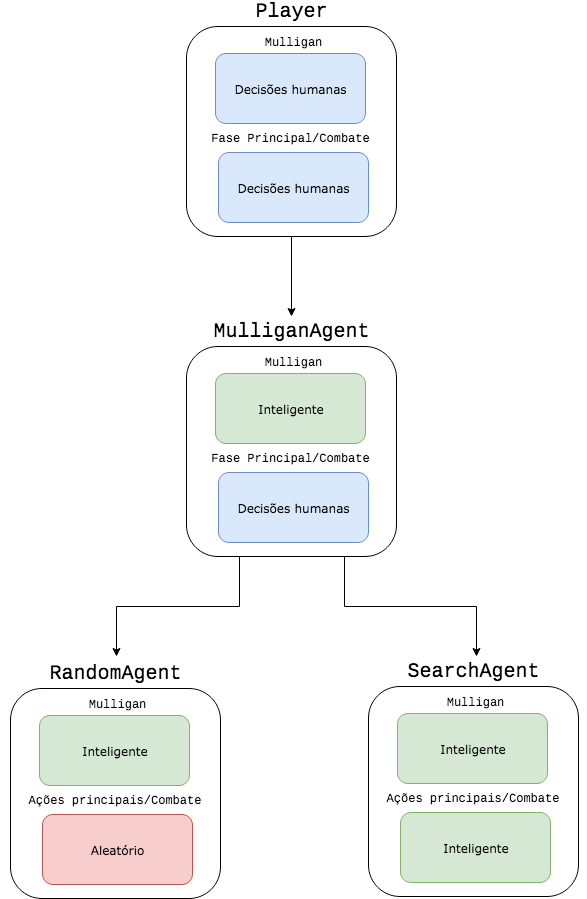
\includegraphics[width=0.6\textwidth]{picstcc/playerdiagram.png}
  \caption{Diagrama de classes de jogadores e agentes.}
  \label{classdiagram}
\end{figure}

Há mais três classes herdadas (diretamente ou não) da classe \texttt{Player}. A primeira delas é \texttt{MulliganAgent}, cuja única diferença funcional em relação a \texttt{Player} é a aplicação de um algoritmo para a decisão automática do mulligan. Um agente \texttt{MulliganAgent} não é 100\% autônomo, pois suas decisões para o resto do jogo ainda são requisitadas ao usuário, e não é chamado pelas opções disponíveis no programa. A existência da classe é justificada pois serve de base para os dois outros agentes (e potencialmente mais): o agente aleatório e o agente inteligente, diferentes entre si. A intenção é que qualquer agente (mesmo aleatório) tenha chance de jogar suas cartas e, para isso, deve definir uma mão inicial suficientemente ``jogável'' (melhor explicado em \ref{sec:mulliganmodel}).
\vskip1ex
A classe \texttt{RandomAgent}, herdada de \texttt{MulliganAgent}, sobrescreve todas as decisões humanas de \texttt{Player} (exceto \texttt{mulligan()}) por métodos que sorteiam e submetem uma ação sorteada dentre a gama de possibilidades. Para isso, usam em cada um de seus métodos um conjunto \texttt{legalActions} de ações legais computado pela instância de \texttt{Game} que os chamou. A obtenção de ações legais é explicada no capítulo \ref{chap:modelagem}.

\vskip1ex
Por fim, a classe \texttt{SearchAgent} também é herdada de \texttt{MulliganAgent} e sobrescreve os métodos de decisões humana por ações decididas por algoritmos. Tais decisões serão examinadas no capítulo \ref{chap:modelagem}.
